
\begin{Large}
\begin{center}
\textbf{Control de versiones} \\
\end{center}
\end{Large}

\section{Control de versiones} 
Se llama control de versiones a la gestión de los diversos cambios que se realizan sobre los elementos de algún producto o una configuración del mismo. Una versión, revisión o edición de un producto, es el estado en el que se encuentra el mismo en un momento dado de su desarrollo o modificación.

Aunque un sistema de control de versiones puede realizarse de forma manual, es muy aconsejable disponer de herramientas que faciliten esta gestión dando lugar a los llamados sistemas de control de versiones o VCS (del inglés Version Control System). Estos sistemas facilitan la administración de las distintas versiones de cada producto desarrollado, así como las posibles especializaciones realizadas (por ejemplo, para algún cliente específico). Ejemplos de este tipo de herramientas son entre otros: CVS, Subversion, SourceSafe, ClearCase, Darcs, Bazaar, Plastic SCM, Git, SCCS, Mercurial, Perforce, Fossil SCM, Team Foundation Server.

\begin{itemize}
	\begin{center}
	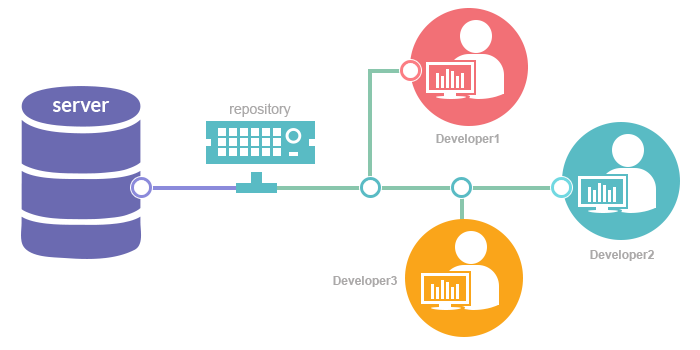
\includegraphics[width=14cm]{./Imagenes/imagen2} 
	\end{center}

	\item Si eres diseñador gráfico o web, y quieres mantener cada versión de una imagen o diseño (algo que sin duda quieres), un sistema de control de versiones (Version Control System o VCS en inglés) es una elección muy sabia. Te permite revertir archivos a un estado anterior, revertir el proyecto entero a un estado anterior, comparar cambios a lo largo del tiempo, ver quién modificó por última vez algo que puede estar causando un problema, quién introdujo un error y cuándo, y mucho más. Usar un VCS también significa generalmente que si fastidias o pierdes archivos, puedes recuperarlos fácilmente. Además, obtienes todos estos beneficios a un coste muy bajo.



\end{itemize} 